\chapter{计算方法}\label{chapter:theory}
% Define abbreviation
\newcommand{\ubm}[1]{\{\bm{#1}\}}

在这一章中,我们将简要介绍凝聚态材料电子结构第一性原理计算所用到的理论方法。重点讨论
密度泛函理论在材料基态性质以及密度泛函微扰理论在晶格动力学性质研究中的应用。
理论原理部分的讨论难以详尽,因此将仅涉及与论文内容相关的概念和讨论。

\section{密度泛函理论}

到目前为止,密度泛函理论(DFT)仍然是用于研究由电子和原子核通过库伦相互作用构成的多体系统的基态性质的最广泛实用的理论方法。该理论由Hohenberg 和 Kohn\cite{hohenberg1964inhomogeneous}于1964年以及Kohn 和 Sham\cite{kohn1965self}于1965年的两篇奠基性工作发展而来。简单来说,根据密度泛函理论,一个系统不但可以通过其多体波函数来完全描述,还可以通过其基态的电子密度来完全描述。体系中电子复杂的多体相互作用中难以处理的部分之间通过对总能贡献的交换相关项进行描述。这一交换相关项的具体形式目前并未被人们知晓,但可以通过如基于自由电子气的模型近似来得到,常见的有局域密度近似(LDA)和广义梯度近似(GGA)。事实上,归功于计算能力的发展,DFT在近几十年中成为真实材料基态性质定量预测的一个极为精确有效的理论工具。

Hohenberg-Kohn(HK)定理描述了这样一个事实,即体系的基态电子密度$n(\bm{r})$与外势$V_\mathrm{ext}$ 之间存在一一对应的关系。
体系的电子密度由其所处的外势唯一确定,同时该电子密度也仅对应于该外势。
因此,体系的能量是电子密度的泛函,该泛函的极小值对应于基态电子密度且给出了正确的基态能量。
然而,多体系统的准确泛函形式并不知晓,密度泛函理论的数值方法的实现基于Kohn-Sham(KS)方法。
KS方法使用一个假想的辅助独立无粒子间相互作用的系统,以构成与真实多体系统相同的电子密度,
从而,将一个有粒子间相互作用的多体问题转化为一组独立粒子与外场势之间可互相自洽求解的问题(类似平均场方法)。
求解体系总能对电子密度泛函的最小极值,可以得到一系列单电子薛定谔方程,即KS方程。多体系统的电子密度因此可以通过求解KS方程(\ref{eq:ks-equation})得到:
\begin{equation}\label{eq:ks-equation}
  \left\{ -\nabla^2 + v_{\mathrm{eff}}(\bm{r}) \right\}\psi_i(\bm{r}) = \epsilon_i \psi_i (\bm{r}),
\end{equation}
$\epsilon_i$是方程的本征值,$\psi_i(\bm{r})$是对应的本征函数,有效势$v_{\mathrm{eff}}$ 是电子密度的泛函,由外势能和诱导的屏蔽势能组成:
\begin{equation}
  v_{\mathrm{eff}}[n] = v_{\mathrm{ext}} + v_{\mathrm{scr}}[n] =
  v_{\mathrm{ext}} + v_{H}[n] + v_{XC}[n],
\end{equation}

电子密度$n(\bm{r})$为:
\begin{equation}
  n(\bm{r}) = \sum_i f_i |\psi_i(\bm{r})|^2 ,
\end{equation}
其中$f_i$为波函数$\psi_i$的占据数。KS方程需要通过自洽的方式求解,因为KS哈密顿量$H^{KS}$中的有效Kohn-Sham势部分$v_{\mathrm{eff}}[n]=v_{\mathrm{ext}} + v_{H}[n] + v_{XC}[n]$是由电子密度所确定的。$v_{\mathrm{ext}}$为电子受到的与原子核间的库伦相互作用,$v_{H}[n]$为电子间的Hatree势,而$v_{XC}[n]$则描述未知的交换-关联势,被定义为交换-关联能对电子密度的泛函微分。在局域密度近似(LDA)中,交换-关联能被认为仅依赖于局域的电子密度,且与均匀的自由电子气模型的交换关联能函数相等。而在广义梯度近似(GGA)中,交换-关联能还依赖于电子密度空间中的梯度。

我们可以看到,KS方法构建了与真实系统相同的基态电子密度和基态总能,但无法定量计算其他的一些性质,
比如,
对于晶格变化导致的外场势变化引起的准粒子态无法单纯通过DFT理论进行描述。

周期性体系数值求解KS方程的常用方法是基于平面波的赝势近似方法。该论文的所有工作均用到这一方法,因此我们将对其进行简要的介绍。

\subsection{赝势近似}
在赝势近似中,我们将核与内层束缚核电子的库伦势作替换将势替换为仅作用于外层价电子的有效势$v^\mathrm{PS}$。
通过近核处平滑的赝波函数,避免了需要过多平面波以描述剧烈振荡的近原子核处真实电子波函数的问题,从而节约了计算成本。
赝势近似前提假定内壳层电子对化学键及化学特性没有重要的影响,且其并不随结构的变化而发生变化,
因此可合理地认为核电子是牢牢固定并静止(frozen)与原子核附近,即静止核近似(frozen core approximation)。这一近似大大节约了计算成本,但代价是赝势在空间中是非局域的,
\begin{equation}
  v^{\mathrm{PS}}(\bm{r},\bm{r'}) = v^{\mathrm{loc}}(\bm{r}) + v^{\mathrm{nl}}(\bm{r},\bm{r'}) ,
\end{equation}
公式中$v^\mathrm{loc}$表示局域贡献的部分,$v^\mathrm{nl}$代表非局域的部分。
第一性原理的赝势来自于原子全电子波函数求解,生成赝势的目标为构建能够几乎完全复现真实原子势散射特性的赝势,
也就是超出特定原子核距离,将真实原子势替换为构建的赝势,依然能解得有完全相同的原子能级本征值。

赝势的种类主要有以下几类:模守恒赝势(NC)\cite{hamann1979norm},
超软赝势(US)\cite{vanderbilt1990soft},
和projecter-augmented wave(PAW)\cite{blochl1994projector}。 
在NC赝势的构建中,要求赝波函数的模与对应的全电子波函数完全相等。
这一条件在US和PAW的构建中适当放宽,从而可以产生更加平滑的赝波函数,
使用较少的平面波基组,
但代价是US赝势和PAW赝势的数学表达更加复杂。

\subsection{平面波基组}
在处理周期性体系时,Kohn-Sham方程满足布洛赫定理,因此波函数可以写为$\psi_{n\bm{k}}(\bm{r})=e^{i\bm{k}\cdot \bm{r}} u_{n\bm{k}}(\bm{r})$的形式,其中$n$和$\bm{k}$分别为能带的索引标号和晶格波矢。函数$u_{n\bm{k}}(\bm{r})$是以晶格为周期的周期函数,满足$u_{n\bm{k}}(\bm{r}+\bm{R})=u_{n\bm{k}}(\bm{r})$,R为晶体的布拉维格子。

在周期性体系中,赝势方法给出的KS方程的数值解波函数可以通过平面波基组展开:
\begin{equation}
  \psi_{n\bm{k}}(\bm{r}) = \sum_{\bm{G}}e^{i(\bm{k}+\bm{G})\cdot \bm{r}}c_{n\bm{k}}(\bm{G}) ,
\end{equation}
其中求和项$G$为倒空间中全部的倒格矢,$c_{n\bm{k}}(\bm{G})$则是对波函数$\psi_{n\bm{k}}(\bm{r})$进行该展开的傅立叶系数。在真实的数值模拟中,我们仅能展开为有限数量平面波,因此对波矢作以下截断:
\begin{equation}
  \frac{|\bm{k} + \bm{G}|^2}{2} < E_{\mathrm{cutoff}} .
\end{equation}
$E_{\mathrm{cutoff}}$是波函数的截断能,该参数控制了展开平面波的数量,也因此影响了计算的精度。
波函数写为平面波基组展开的形式,KS方程$H\left|\psi_i\right>=\epsilon_i\left|\psi_i\right>$可写为矩阵形式的久期方程,本征值和本征波函数可通过迭代对角化得到。

\subsection{绝热近似}\label{sec:BO-approx}

我们考虑固体由电子和离子组成,此处的离子是原子核和非价层的核电子组成的统一整体。晶体中电子和离子的动力学可以由以下哈密顿量描述:
\begin{equation}
  \mathcal{H} = T_e + V_{ee} + T_i + V_{ii} + H_{e-i} ,
\end{equation}
其中$T_e$和$T_i$分别是电子和离子的动能项,$ V_{ee}$,$V_{ii}$分别表示电子和离子之间的库伦相互作用势,$H_{e-i}$则概括了电子和离子的相互作用。

由于电子的质量远远小于离子的质量,我们可以认为较轻的电子比更重的离子以快的多的速度移动,
从而近似对耦合的多体薛定谔方程$\mathcal{H} \Psi(\ubm{r},\ubm{R})=\mathcal{\varepsilon} \Psi(\ubm{r},\ubm{R})$ (花括号用于表示一组粒子的坐标)
进行简化而使得方程可以数值解。我们认为在离子发生振动产生移动后,
电子几乎瞬间发生了重新排布。这样的现象可以通过引入微扰参数$\kappa$来描述离子产生的位移,
在离子质量趋向于无穷大$M\rightarrow+\infty$时,该参数趋向于$\kappa\rightarrow 0$,这个描述最早由Born和Oppenheimer\cite{oppenheimer1927quantum}用于分子的振动,
并由Chester和Houghton\cite{chester1959electron}拓展到对固体(周期性)的描述。

设离子振动偏移平衡位置:
\begin{equation}
  \bm{R}_i = \bm{R}^0_i + \kappa \bm{u}_i .
\end{equation}

动能项中参数$\kappa$指数项为\num{-2},势能项该参数指数项为\num{2},
令动能项和势能项该参数的阶相等,则得到$\kappa$的形式为:$\kappa=(m/M)^{1/4}$,
该参数除了对氢和氦两种元素,值均小于\num{0.1}。
使用这个参数,可以用微扰法对哈密顿量和波函数进行系统的展开。
最低阶项展开式中波函数可以写为$\Psi(\ubm{r},\ubm{R})=\chi(\ubm{R})\psi(\ubm{r};\ubm{R})$,
可以看到电子波函数仅参数地依赖于原子坐标。因此电子波函数满足方程:
\begin{equation}\label{eq:dfpt_ele_eigen}
  \left[ T_e + V_{ee} + H_{e-i}(\ubm{R}) \right]\psi_n(\ubm{r};\ubm{R}) = E_n(\ubm{R})\psi_n(\ubm{r}; \ubm{R}) .
\end{equation}

对离子位置R的依赖统一通过$H_{e-i}$描述,离子的位置是下列方程的解:
\begin{equation}\label{eq:dfpt_ion_eigen}
  \left[ T_i + V_{ii} + E_n(\ubm{R}) \right] \chi(\ubm{R}) = \xi \chi(\ubm{R}) .
\end{equation}

这个近似被称为绝热近似或Born-Oppenheimer近似。
该近似将电子和离子进行了动力学的解耦,
忽略了离子移动导致的电子的激发。式(\ref{eq:dfpt_ion_eigen})中,
$E_n$是电子系统的某个本征值,通常可认为是解耦后电子薛定谔方程式(\ref{eq:dfpt_ele_eigen})的基态解,
而且,有限温度的电子激发通常不会对离子移动造成影响。
% 这一项包含了重要的价电子对离子实移动的屏蔽效应,虽然该效应对基态和对激发态是一样的。

\section{密度泛函微扰理论}

任何固体物质都包含了电子和声子这两种元激发。
对固态物质性质的本质的理解都基于对电子和声子这两种准粒子的清晰认识。
然而,要解出周期性体系中电子和原子核(或将原子核和内层非价电子构成的离子看作独立的对象)
互相耦合的多体量子力学问题是一个接近不可能的任务。但由于电子和原子核在质量上的巨大差别,
它们两者可以近似地看作独立的两个动力学子系统而独立求解。
近几十年,快速发展的数值方法,使得从第一性原理求解电子部分的量子问题成为可能。
大多数的第一性原理求解电子量子问题的方法都是基于上一节所描述的密度泛函的方法,
现在有许多DFT的软件,使得电子结构的求解成为物质研究的一个例行的探索步骤。
对声子部分的第一性原理求解的方法的成熟比电子部分的更晚,
这是因为对基础的振动性质的精确的数值描述是要以精确的电子结构的描述为基础的。
上世纪90年代所发展的通过微扰的线性响应的方法,也就是题目中的密度泛函微扰理论(DFPT)现在已经成为准确地描述声子的高效的数值方法。

电子和声子之间的相互作用即电声耦合,影响甚至主导了许多固相物质的物理性质。
该相互作用最明显的例子是,在金属中,晶格振动影响了低能级的电子激发,
从而导致了可观测的电子迁移性质和热力学性质的改变。
而且,电声耦合是电子自发成对的原因之一,这导致了超导这一宏观的物理现象。

这一节我们将介绍DFT框架下,第一性原理数值求解电声耦合的方法。
% 再过渡到声子调制的电子成对相互作用从而得以描述超导电性。
在开始,有必要先简要叙述并给出一些数学描述以方便后续的介绍。
这部分的剩余内容将紧接着\ref{sec:BO-approx}小结的绝热近似,
给出比绝热近似更精确的描述,再进一步介绍晶格振动的唯像描述。

为得到比以上\ref{sec:BO-approx}小节绝热近似更精确的解,我们使用式(\ref{eq:dfpt_ele_eigen})的波函数解为基组来展开原系统的波函数:
\begin{equation}\label{eq:psi_mix}
  \Psi_m(\ubm{r};\ubm{R}) = \sum_n \chi_{mn}(\ubm{R})\psi_n(\ubm{r};\ubm{R}).
\end{equation}

将式\ref{eq:psi_mix}代入系统薛定谔方程$\mathcal{H} \Psi_m(\bm{r},\bm{R})=\mathcal{\varepsilon}_m \Psi_m(\bm{r},\bm{R})$整理得到离子部分满足方程:
\begin{equation}
  \left[ T_i + V_{ii} + E_n(\ubm{R}) \right] \chi_{mn}(\ubm{R}) + \sum_{n'}\Delta H_{nn'}\chi_{mn'}(\ubm{R}) = \xi_m \chi_{mn} (\ubm{R}) ,
\end{equation}
与绝热近似时离子位置满足的方程式(\ref{eq:dfpt_ion_eigen})相比多出了左边第二项,其中$\Delta H=\Delta H^{(1)} + \Delta H^{(2)}$:
\begin{equation}
  \Delta H_{nn'}^{(1)} = -\frac{1}{M}\sum_i \int dr^{3N}\psi_n^*(\ubm{r};\ubm{R})\nabla_{R_i}\psi_{n'}(\ubm{r};\ubm{R})\cdot \nabla_{R_i} ,
\end{equation}
\begin{equation}时
  \Delta H_{nn'}^{(2)} = -\frac{1}{2M}\sum_i \int dr^{3N}\psi_n^*(\ubm{r};\ubm{R})\nabla^2_{R_i}\psi_{n'}(\ubm{r};\ubm{R}) .
\end{equation}

这两项中都有电子波函数对离子实位置的偏导,
因此包含了离子实位置移动所导致的电子子系统的激发情况。
第一项展开的系数为$\kappa$,第二项为$\kappa^2$,同时由于$\kappa$值很小(除原子质量最小的几个原子需要特别考虑),
因此第一项的值远大于第二项,主导了非绝热过程。
非绝热修正项对结果波函数的影响为$\kappa^3$,对能量的影响为$\kappa^6$。$\kappa$的
值仅依赖于质量比而与电子离子相互作用的强度无关。
综上绝热近似无论对于近自由电子的系统还是价电子束缚在离子实周围的体系都适用。
在绝热近似下,我们通过以下有效势来给出离子的受力以及动力学结果:
\begin{equation}\label{eq:effective_potential}
  \Omega(\ubm{R}) = V_{ii}(\ubm{R}) + E_0(\ubm{R}),
\end{equation}
其中$E_0(\ubm{R})$是给定的一组离子坐标$\ubm{R}$下的电子基态能量。
经典的教材\cite{born1954dynamical,bottger1983principles}(晶格动力学部分章节)
都是从这个有效势$\Omega$开始来构建晶格动力学的微观理论。

我们通过对势能$\Omega$在参考位置$\ubm{R}^0$附近位移$u$来进行展开以得到系统动力学性质:

\begin{equation}
  \Omega(\ubm{R}) = \Omega(\ubm{R}^0) + \sum_{i\alpha} \Phi_\alpha(i)u_{i\alpha} + \frac{1}{2} \sum_{i\alpha j\beta} \Phi_{\alpha\beta}(i,j) u_{i\alpha}u_{j\beta} + \cdots ,
\end{equation}
希腊字母$\alpha$和$\beta$描述的是离子的空间笛卡尔坐标序号即$x,y,z$,$i$和$j$是原子的序号。一次项的系数$\Phi_\alpha$是作用在参考原子上的力的相反数:

\begin{equation}
  F_{i\alpha} = -\frac{\partial\Omega}{\partial R_{i\alpha}}\bigg|_0 = -\Phi_\alpha(i) ,
\end{equation}
如果我们选择参考位置为平衡位置,则此时该项为零,且平衡位置处势能$\Omega$达到极小值。
二次项系数为:

\begin{equation}\label{eq:omega_second_order}
  \Phi_{\alpha\beta} = \frac{\partial^2\Omega}{\partial R_{i\alpha}\partial R_{j\beta}} \bigg|_0 ,
\end{equation}
这一系数的物理意义为,第$i$个原子偏离平衡位置所导致的第$j$个原子感受到的力的变化:

\begin{equation}
  F_{j\beta} = -\sum_{i\alpha} \Phi_{\alpha\beta}(i,j)u_{i\alpha} ,
\end{equation}

该项描述了位移随力的线性变化。
也就是弹簧振子的简谐振动力常数的三维(张量)版本。
如果仅截断到二次项,就是我们常说的简谐近似。更高次项系数被称为非简谐力常数。在周期性体系中,
原子的序号可以使用一对符号来表示即:$i=(l\kappa)$,
其中$l$表示单胞序号,$\kappa$表示原子在单胞内的序号。

通过傅立叶变化将力常数矩阵变换到倒空间为动力学矩阵:

\begin{equation}
  D_{\kappa\alpha\kappa'\beta}(\bm{q}) = \frac{1}{\sqrt{M_\kappa M_{\kappa'}}} \sum_l \Phi_{\alpha\beta}(l\kappa,0\kappa')e^{-i\bm{q}(\bm{R}^0_{l\kappa}-\bm{R}^0_{0\kappa'})} ,
\end{equation}
该矩阵决定了晶体中的振动模式即所谓的声子,

\begin{equation}
  \sum_{\kappa'\beta}D_{\kappa\alpha\kappa'\beta}(\bm{q})\eta_{\kappa'\beta}(\bm{q}j) = \omega^2_{\bm{q}j}\eta_{\kappa\alpha}(\bm{q}j) ,
\end{equation}
其中$\omega^{\bm{q}j}$和$\eta_{\kappa\alpha}(\bm{q}j)$分别是确定波矢$\bm{q}$第分支$j$的频率和振动模式。

% 通过这两个量可以建立原子位移和声子之间的联系,设声子的升降算符为$b$和$b^{\dagger}$,则:

% \begin{equation}
%   u_{l\kappa\alpha} = e^{i\bm{q}\bm{R}^0_{l\kappa}}\frac{1}{\sqrt{N_q}} \sum_{\bm{q}j} A^{\bm{q}j}_{\kappa\alpha}(b_{\bm{q}j} + b^{\dagger}_{-\bm{q}j}) ,
% \end{equation}

% 其中:

% \begin{equation}
%   A^{\bm{q}j}_{\kappa\alpha} = \frac{\eta_{\kappa\alpha}(\bm{q}j)}{\sqrt{2M_\kappa \omega_{\bm{q}j}}} .
% \end{equation}

% 要完全的描述简谐振动的谱性质,需要知道全布里渊区的振动模式信息,
% 或者知道实空间中所有原子键之间的力常数。
% 在金属材料中,由于电子对离子移动的屏蔽,
% 实空间中晶格间的键的相互作用很小,可以在比较小的距离截断,因而使用力常数的描述更节约计算资源。

\subsection{第一性原理晶格动力学}
晶格动力学首先要计算决定离子动力学性质的力学量。式(\ref{eq:effective_potential})中
有效势$\Omega$可拆分为左边两项,第一项$V_{ii}$是离子间的库伦相互作用,
可以直接得到其对力常数的贡献;第二项$E_0$综合了由电子贡献的与键和电子对离子屏蔽的相关物理量的信息,
该项需要通过准确的电子结构计算来给出,可以通过密度泛函理论(DFT)对体系基态求解实现。

晶格势决定了晶格的动力学性质,而晶格势等于固定原子位置后构型的基态能量,该能量可以通过DFT求解。
从第一性原理求解晶格动力学性质主要可以分为两类方法\cite{fritsch1999density}:
1)直接求解力矩阵,2)线性响应法。直接法是通过计算理想晶格以及计算特定的原子移动后的构型能量来得到力矩阵。
冷冻声子法(FP)是概念上最为简单且最早被使用直接求力矩阵的方法,
它通过能量和位移的二次关系来提取振动模式及模式的频率\cite{yin1980microscopic}。
这个方法需要首先确定声子的本征函数从而知道如何移动原子,
因此该方法需要提前知道晶体的对称性信息。
但由于FP方法中对原子移动了有限的距离,因此它可以包含非简谐的效应,
可以通过拟合能量和力的高阶关系用来计算更高阶的系数。
通过移动个别原子后其他单胞内原子受力改变和移动原子距离的线性关系来计算晶格性质是
更为高效的一个方法。通过海尔曼-费曼定理,
即原子受力可以直接从移动原子后体系基态求解过程中得到(不需要作能量对位置偏导)。
因此对应一个原子的移动只需要简单的计算就可以给出动力学矩阵的一行,
合适地选取原子位移,就能够得到整个动力学矩阵。该方法并不需要提前得到晶体的对称性信息。
和线性响应法相比,直接法的缺点是如果要求解非零波矢的声子(除$\Gamma$点外)性质,
需要构建超胞,如果要得到完整的声子谱,则超胞需要大到晶格单胞之间的相互作用可以忽略不计\cite{frank1995ab,kresse1995ab}。
线性响应法通过微扰的方法来计算能量的导数,
力学矩阵可以从二阶偏导,公式(\ref{eq:omega_second_order})直接得到。
使用这个方法,无需构建超胞就能直接在倒空间任意波矢求解从而获得完整的动力学性质\cite{baroni2001phonons}。
因为在本论文工作的稳定性确定和超导计算部分用到了这一方法,我们在下面详细描述该方法。

\subsection{DFPT计算声子性质}
本小节我们给出在DFT框架下周期体系基于对原子位置微扰的方法求动力学矩阵的详细过程。
首先我们假设这样的情况,即外场势$v_{\mathrm{ext}}$依赖于
一组绝热的微扰参数$\Lambda={\lambda_a,\lambda_b, \cdots \lambda_p}$,
每个外势$v_{\mathrm{ext}}^\Lambda$对应一个电子密度和确定的总能
\begin{equation}
  E^\Lambda = F[n^\Lambda]+\int d^3 r n^\Lambda (\bm{r})v_\mathrm{ext}^\Lambda (\bm{r}) ,
\end{equation}

因此加外势扰动后总能对微扰参数的偏导为:
\begin{equation}
  \frac{\partial E^\Lambda}{\partial \lambda_a} =
  \int d^3 r n^\Lambda(\bm{r})\frac{\partial v^\Lambda_\mathrm{ext}(\ubm{r})}{\partial \lambda_a} +
  \int d^3 r \frac{\delta E^\Lambda}{\delta n(\bm{r})} \frac{\partial n^\Lambda(\bm{r})}{\partial \lambda_a} ,
\end{equation}

第二项的电子密度为势能量最小的基态电子密度,由变分法可知第二项为零。而这就是DFT框架下的海尔曼-费曼定理\cite{feynman1939forces}。微扰后能量的二阶偏导为:
\begin{equation}\label{eq:second_order_energy}
  \frac{\partial^2 E^\Lambda}{\partial\lambda_a\partial\lambda_b} =
  \int d^3 r\frac{\partial n^\Lambda(\bm{r})}{\partial\lambda_b}\frac{\partial v^\Lambda_\mathrm{ext}(\bm{r})}{\partial\lambda_a} +
  \int d^3 r n^\Lambda(\bm{r})\frac{\partial^2 v^\Lambda_\mathrm{ext}(\bm{r})}{\partial\lambda_a\partial\lambda_b} ,
\end{equation}

从上式可知,要求解能量的二阶导只需要得到关于电子密度的一阶导。因此仅需要考虑系统对微扰的线性响应。有效势在微扰后可以写成以下形式:
\begin{equation}\label{eq:linear_variation}
  \delta v_{\mathrm{eff}}(\bm{r}) = \delta v_\mathrm{ext}(\bm{r}) + \delta v_\mathrm{scr}(\bm{r}) =
  \delta v_\mathrm{ext}(\bm{r}) + \int d^3 r' I(\bm{r},\bm{r'})\delta n(\bm{r'}) ,
\end{equation}

\begin{equation}
  I(\bm{r},\bm{r'}) \equiv \frac{\delta v_\mathrm{scr}(\bm{r})}{\delta n(\bm{r'})} = \frac{\delta v_H(\bm{r})}{\delta n(\bm{r'})} +
  \frac{\delta v_{XC}(\bm{r})}{\delta n(\bm{r'})} =
  \frac{2}{|r-r'|} + \frac{\delta^2 E_{XC}}{\delta n(\bm{r}) \delta n(\bm{r'})} ,
\end{equation}

使用微扰原理,KS波函数的一阶变分为:
\begin{equation}
  \delta \psi_i(\bm{r}) = \sum_{\substack{i,j\\i\neq j}} \frac{\langle i |\delta v_{\mathrm{eff}}|j \rangle}{\epsilon_i-\epsilon_j} \psi_j(\bm{r}) ,
\end{equation}

同样写出$\delta \psi_i^*(\bm{r})$可以得到电子密度的一阶变分为:
\begin{align}\label{eq:linear_variation_ele}
  \delta n(\bm{r}) &= \sum_i f_i [\psi_i^*(\bm{r})\delta \psi_i(\bm{r}) + \delta \psi_i^*(\bm{r}) \psi_i(\bm{r})] \\
  &= \sum_{i\neq j} \frac{f_i-f_j}{\epsilon_i-\epsilon_j} \langle j| \delta v_\mathrm{eff} | i \rangle \psi_i^*(\bm{r}) \psi_j(\bm{r}) ,
\end{align}

从公式(\ref{eq:linear_variation})和公式(\ref{eq:linear_variation_ele})可以发现
,$\delta n$和$\delta v_\mathrm{eff}$互相依赖,需要通过自洽法求解。
接着为了凸显电子密度随有效势$\delta v_\mathrm{eff}$的变化关系我们还可以把以上关系写为:
\begin{equation}
  \delta n(\bm{r}) = \int d^3 r' \chi_0 (\bm{r},\bm{r'})\delta v_\mathrm{eff}(\bm{r'}) ,
\end{equation}
\begin{equation}
  \chi_0(\bm{r},\bm{r'}) = \sum_{i\neq j}\frac{f_i-f_j}{\epsilon_i-\epsilon_j} \psi^*_i(\bm{r})\psi_j(\bm{r})\psi^*_j(\bm{r'})\psi_i(\bm{r'}) ,
\end{equation}

此处的$\chi_0$是无相互作用的KS系统的电极化率,它仅仅依赖于系统基态。
虽然使用微扰方法,但由于处理的是电子无相互作用的KS系统,因此没有更高阶的近似。
现在已知有效势对电子密度的影响,要得到电子密度和外势之间的关系,
我们使用式(\ref{eq:linear_variation})有效势可以写为:

\begin{align}
  \delta v_\mathrm{eff} &= \delta v_\mathrm{ext} + I \chi_0 \delta v_\mathrm{eff} \\
  &= [1-I\chi_0]^{-1} \delta v_\mathrm{ext} = \epsilon^{-1} \delta v_\mathrm{ext} ,
\end{align}
其中$\epsilon$为静态介电常数矩阵,描述的是体系对外场微扰的屏蔽。

为高效求解该介电常数矩阵的逆就引出了本章所要介绍的方法DFPT,
其克服了许多其他方法的不足,如求解$\chi_0$时需要未占据态,
以及对于周期体系实空间中的介电矩阵为无穷维,
通过傅立叶变换到倒空间该矩阵逆的求解十分耗费计算资源。
DFPT通过自洽法来实现线性响应法而避免了介电常数矩阵求解时的困难。

公式(\ref{eq:linear_variation_ele})电子密度的一阶变分中包含了对电子态的两次的求和,
而参数$(f_i-f_j)/(\epsilon_i-\epsilon_j)$限制了(这仅限于对半导体,
对金属的拓展可参考文献\cite{de1995lattice})其中一个态为导带另一个态来自价带,
不考虑磁性时体系满足时间反演对称性,式(\ref{eq:linear_variation_ele})可以写为:

\begin{equation}
  \delta n(\bm{r}) = 2\sum_{vc}\frac{1}{\varepsilon_v-\varepsilon_c}
  \langle c| \delta v_\mathrm{eff} | v\rangle \psi^*_v(\bm{r})\psi_c(\bm{r}) ,
\end{equation}
整理并把导带部分写在一起后得:

\begin{equation}\label{eq:delta_n_valence}
  \delta n(\bm{r}) = 2\sum_v \psi^*_v(\bm{r}) \Delta_v(\bm{r}) ,
\end{equation}
\begin{equation}
  |\Delta_v \rangle = \sum_{c}\frac{1}{\varepsilon_v-\varepsilon_c}
  |c\rangle \langle c| \delta v_\mathrm{eff} | v\rangle ,
\end{equation}
该右矢$|\Delta_v\rangle$满足下列线性方程:

\begin{equation}
  (H-\epsilon_v)|\Delta_v\rangle = -\sum_c |c\rangle \langle c| \delta v_\mathrm{eff} | v\rangle = (P_v-1)\delta_\mathrm{eff}|v\rangle ,
\end{equation}

因此,给定$\delta v_\mathrm{eff}$可以从上述线性方程组
求得$|\Delta_v\rangle$,代回(\ref{eq:delta_n_valence})
可以得到$\delta n$,进而能得到新的$\delta v_\mathrm{eff}$。
自洽得到最后的结果。用该自洽方法求解外场对电子密度的扰动{\textbf{不需要}}用到导带部分的信息。

这里我们用DFPT来计算原子间力常数。
将全实空间的偏离平衡位置的位移写成下列函数的形式,
从而可以描述特定声子对应实空间的不同单胞的原子的位移:

\begin{equation}
  u_{l\kappa\alpha} = d_{\kappa\alpha}e^{i\bm{q}\bm{R}^0_{l\kappa}} + d^*_{\kappa\alpha}e^{-i\bm{q}\bm{R}^0_{l\kappa}} ,
\end{equation}

其中$l$是单胞的序号,$\kappa$是单胞内的某个原子,$\alpha$是笛卡尔坐标序号$x$,$y$或$z$。
复数表示的振幅$d_{\kappa\alpha}$使得可以包含特定的原子位移的相对相位。
电子对结构的动力学特性有这样的影响,
即当晶体中原子振动造成原子所构成的外势的改变,
外势的改变又使得电子快速重新排列,
新的电子结构的改变对原子又产生了新的力的作用。
因此,我们可以将上述作用通过这样的关系表述,
电子部分对动力学矩阵的贡献为:

\begin{equation}\label{eq:Dmatrix}
  D_{\kappa\alpha\kappa'\beta}(\bm{q}) =
  \frac{1}{\sqrt{M_\kappa M_{\kappa'}}} \delta^{\bm{q}}_{\kappa\alpha} \delta^{-\bm{q}}_{\kappa'\beta} E \bigg|_{\bm{u}=0} ,
\end{equation}

\begin{equation}\label{eq:Edd}
  \delta^{\bm{q}}_{\kappa\alpha}\delta^{-\bm{q}}_{\kappa'\beta} E =
  \sum_{\bm{G}} [ \delta^{\bm{q}}_{\kappa\alpha}n(\bm{G}+\bm{q})\delta^{\bm{-q}}_{\kappa'\beta}v_\mathrm{ext}(\bm{G}+\bm{q}) + \delta^{\bm{q}}_{\kappa\alpha}\delta^{\bm{-q}}_{\kappa'\beta} v_\mathrm{ext}(\bm{G})] .
\end{equation}

其中$\delta^{\bm{q}_{\kappa\alpha}}\equiv \frac{\partial}{\partial d_{\kappa\alpha}}$以及
$\delta^{\bm{-q}_{\kappa'\beta}}\equiv \frac{\partial}{\partial d^*_{\kappa\alpha}}$。
使用式(\ref{eq:second_order_energy}),动力学矩阵可以分为两部分,即来自于离子势的二阶偏导和电子的一阶偏导所贡献的屏蔽部分。
通常在晶体中,外势可以写为由原子势叠加而成的形式:
\begin{equation}
  v_\mathrm{ext}(\bm{r}) = \sum_{l\kappa} v_\kappa (\bm{r}-\bm{R}_{l\kappa}).
\end{equation}

平衡位置处,外势的一阶偏导的值为:
\begin{align}
  \delta^{\bm{q}}_{\kappa\alpha}v_{\mathrm{ext}}(\bm{r}) &=
  - \sum_l \nabla^{\bm{r}}_\alpha v_\kappa (\bm{r}-\bm{R}^0_{l\kappa})e^{i\bm{q}\bm{R}^0_{l\kappa}} \\
  &= -e^{i\bm{qr}} \sum_l e^{i\bm{q} (\bm{R}^0_{l\kappa}-\bm{r})} \nabla^{\bm{r}}_\alpha v_\kappa(\bm{r}-\bm{R}^0_{l\kappa}) ,
\end{align}

而电子部分,则就需要通过DFPT方法求得。
即首先将电子密度的变分通过傅里叶变换到倒空间,
同样将其写为导带部分的求和形式,如公式\ref{eq:delta_n_valence},
再通过求解非齐次线性方程组获得每个外势所对应的右矢$| \Delta^{\bm{q}}_{\kappa\alpha}(\bm{k}v) \rangle$后,
代回求下一个循环的新的电子密度的偏导。

\begin{equation}\label{eq:dfpt_scf01}
  \delta^{\bm{q}}_{\kappa\alpha} n(\bm{q}+\bm{G}) = - \frac{4}{V}\sum_{\bm{k}v} \langle \bm{k}v| e^{-i(\bm{q}+\bm{G})\bm{r}}| \Delta^{\bm{q}}_{\kappa\alpha}(\bm{k}v) \rangle ,
\end{equation}
% $V$为晶体的单胞体积,其中的$|\Delta^{\bm{q}}_{\kappa\alpha}(\bm{k}v) \rangle$即为式(\ref{eq:delta_n_valence})中的部分,
% 定义如下:
\begin{equation}\label{eq:dfpt_scf02}
  | \Delta^{\bm{q}}_{\kappa\alpha}(\bm{k}v) \rangle =
  \sum_c \frac{|\bm{k}+\bm{q}c\rangle \langle \bm{k}+\bm{q}c | \delta^{\bm{q}}_{\kappa\alpha} v_\mathrm{eff} | \bm{k}v \rangle}
  {\epsilon_c(\bm{k}+\bm{q})-\epsilon_v(\bm{k})} ,
\end{equation}
\begin{equation}\label{eq:dfpt_scf03}
  (H^{\bm{k}+\bm{q}}_{KS}-\epsilon_v(\bm{k}))|\Delta^{\bm{q}}_{\kappa\alpha}(\bm{k}v)\rangle =
  (P^{\bm{k}+\bm{q}}_v-1)\delta^{\bm{q}}_{\kappa\alpha}v_\mathrm{eff}|\bm{k}v\rangle ,
\end{equation}

三个方程可以自洽求解。
自洽后得到特定倒空间点$\bm{q}$的电子和外势$v_\mathrm{eff}$的变分,
从而可代入\ref{eq:Dmatrix}求解该$\bm{q}$点处的动力学矩阵得对应的声子模式。

% 式(\ref{eq:dfpt_scf01}),式(\ref{eq:dfpt_scf02})和式(\ref{eq:dfpt_scf03})组成的

上述方法已经在许多的第一性原理软件包中实现,
比如,我们可以计算\ce{Si}的声子谱,其结果如图\ref{fig:pd}所示:

\begin{figure}[H]
  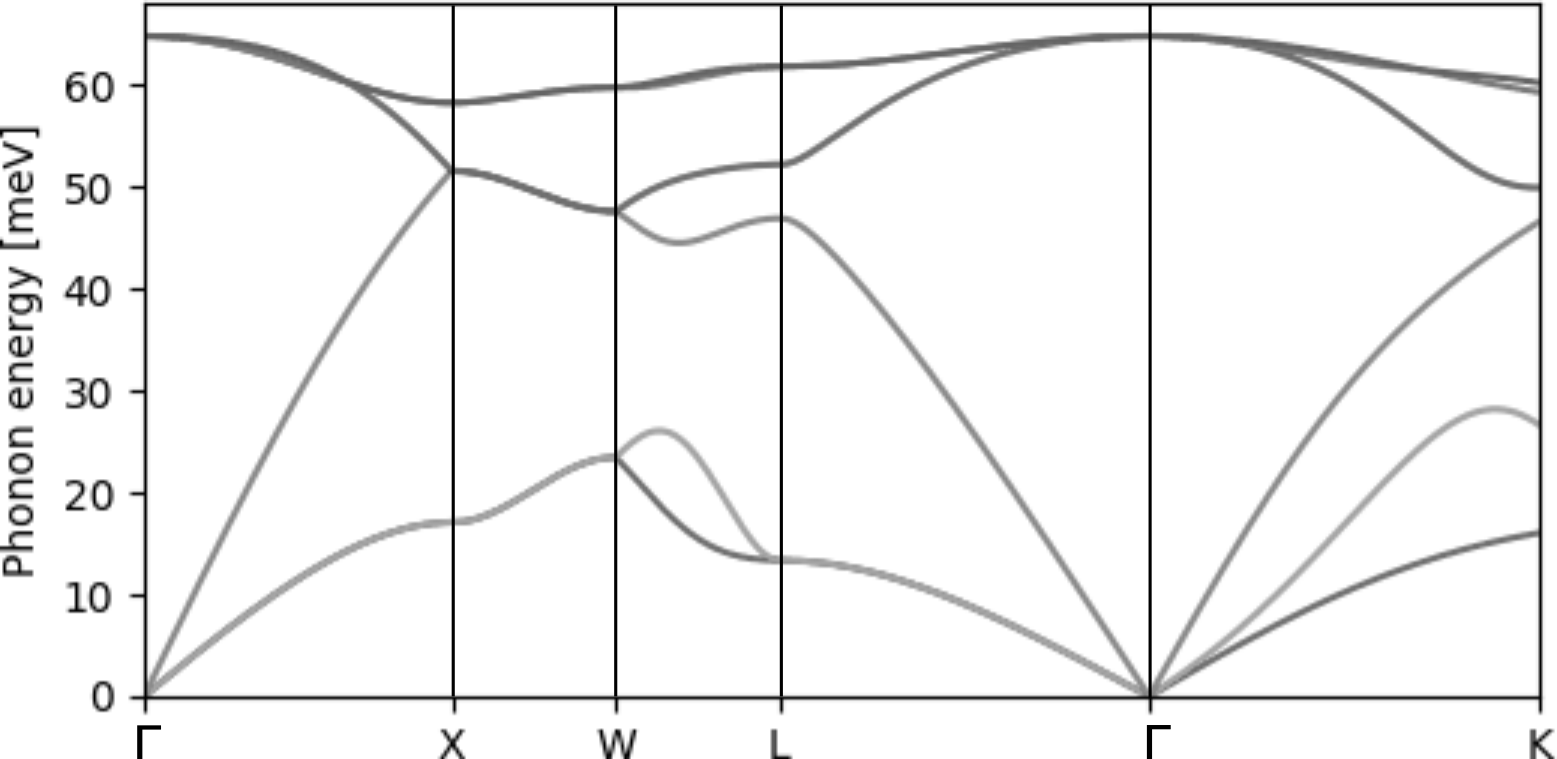
\includegraphics[width=0.82\textwidth]{figs/gray-pd.png}
  \centering
  \caption{\ce{Si}的声子谱}
  \label{fig:pd}
\end{figure}

在该声子谱的计算中,
我们选取的高对称点路径为$\Gamma-X-W-L-\Gamma-K$。
图中的横坐标为倒空间中的点,对应理论公式的记号$\bm{q}$,
在数值计算时,所有的$\bm{q}$之间是互相独立的,因此可以并行计算。
每一个$\bm{q}$值能够计算得到一个动力学矩阵$D_{\kappa\alpha\kappa'\beta}(\bm{q})$,
对该矩阵对角化后本征值就是每一个声子模式的能量,对应图中的纵坐标点。
本征函数就代表对应声子的振动模式。

